\section{Resolución}

Tenemos $k$ calles bidireccionales a comparar y buscamos de entre ellas la que minimice el valor del camino más corto entre $s$ y $t$ en caso de construirla. Este problema puede ser modelado con un digrafo, donde todo par de puntos está conectado por a lo sumo una arista dirigida. Luego, $s$ y $t$ contarán, o no, con un camino mínimo original el cual buscamos mejorar, o crear, agregando las aristas correspondientes a las calles bidireccionales propuestas. Proponemos entonces el siguiente algoritmo:

\begin{enumerate}
    \item Armamos un digrafo que modele a la ciudad, donde cada punto es un nodo y cada calle unidireccional es una arista. 
    \item Utilizamos el algoritmo de Dijkstra para encontrar los caminos mínimos desde $s$ hacia todos los nodos.
    \item Dando vuelta las aristas, utilizamos el algoritmo de Dijkstra para encontrar el camino mínimo de todos los nodos hacia $t$ en el digrafo original.
    \item Por cada arista bidireccional $k_i$ de largo $l(k_i)$ que une a dos puntos $v$ y $w$, y sea $d(u,p)$ la longitud del camino más corto entre los vértices $u$ y $p$, buscamos la que minimice:
     $$min(\ d(s,t),\ d(s,v) + l(k_i) + d(w,t),\ d(s,w) + l(k_i) + d(v,t)\ )$$
    \item Devolver la longitud mínima.
\end{enumerate}


La idea detrás del algoritmo es considerar todas las calles posibles a construir sin tener que recalcular el nuevo camino mínimo entre $s$ y $t$ con el algoritmo de Dijkstra por cada una. Entonces, luego de obtener los mejores caminos desde $s$ hacia todos los nodos, y desde todos los nodos hacia $t$, podemos rápidamente obtener la longitud del nuevo camino más corto luego de construir la calle $k_i$ con las fórmulas mencionadas en el paso 4. 


\subsection{Demostración de Correctitud}
\vspace{1em}

Queremos ver que el algoritmo devuelve una solución válida y óptima. Por un lado, buscamos probar que la solución que obtiene es uno de los caminos mínimos entre $s$ y $t$, en caso de agregar alguna de las $k$ calles bidireccionales posibles a la ciudad. Por otro lado, queremos ver que no existe un resultado mejor. Es decir, para cualquier otro camino mínimo entre $s$ y $t$ con el agregado de una calle a la ciudad, su longitud será igual o mayor a la devuelta.

\vspace{1em}

Demostremos todo esto haciendo inducción sobre el invariante del algoritmo. Observando el mismo, se puede apreciar que luego de $i$ pasos, se habrán considerado las primeras $i$ calles posibles a construir, y se tiene almacenada la longitud del camino más corto entre $s$ y $t$ luego de haber construido una de ellas. Llamemos la variable que guarda este valor $mn$. 

\vspace{1em}

\textbf{Caso base:} Cuando $i = 0$, no se consideró todavía ninguna calle bidireccional y $mn$ almacena el mejor camino entre $s$ y $t$ en el digrafo original. Entonces, se cumple triviálmente el invariante.

\vspace{1em}

\textbf{Paso Inductivo:} Supongamos que luego de $i$ pasos del algoritmo se consideraron las primeras $i$ calles bidireccionales, y se tiene almacenada la longitud del mejor camino entre $s$ y $t$ habiendo construido alguna de ellas. Buscamos probar que, luego del paso $i+1$, se consideró la siguiente calle y se actualizó correctamente el valor almacenado.

\vspace{1em}

En este paso, se considera la calle bidireccional $k_{i+1}$ que tiene longitud $l(k_{i+1})$ y conecta a los puntos $v$ y $w$. Luego, el algoritmo toma la menor de entre las siguientes tres longitudes posibles:

\begin{itemize}
        \item La ya almacenada en $mn$.
        \item Ir desde $s$ hasta $v$ con longitud mínima, viajar a $w$, y desde $w$ hasta $t$ con longitud mínima, con costo $d(s,v) + l(k_{i+1}) + d(w,t)$.
        \item Ir desde $s$ hasta $w$ con longitud mínima, viajar a $v$, y desde $v$ hasta $t$ con longitud mínima, con costo $d(s,w) + l(k_{i+1}) + d(v,t)$.
\end{itemize}

De ser $mn$ el menor de los tres, por hipótesis inductiva, esta es la longitud del mejor camino mínimo entre $s$ y $t$ hasta el momento, con lo cual se cumple que $mn$ sigue siendo el mejor luego de $i+1$ pasos.

\vspace{1em}

Ahora, pensemos que pasa cuando el mínimo es uno de los dos nuevos caminos que pasan por la calle bidireccional $k_{i+1}$. Por hipótesis inductiva, como $mn$ es la longitud del mejor camino mínimo hasta ahora, este nuevo camino es mejor que todos los anteriores. Luego, solo queda ver que en el digrafo donde se agregaron las aristas $v \rightarrow w$ y $w \rightarrow v$, sea efectivamente uno mínimo entre $s$ y $t$. 

\vspace{1em}

En este digrafo, como se mejoró el camino mínimo con respecto al original, el nuevo camino mínimo debe necesariamente pasar por alguna de las dos aristas agregadas. Luego, su longitud debe ser igual a $min(\ d(s,v) + l(k_i) + d(w,t),\ d(s,w) + l(k_i) + d(v,t)\ )$. Esto es porque esta fórmula representa la distancia del camino mínimo incluyendo alguna de las nuevas aristas, ya que sabemos que una arista, en caso de ser st-eficiente, debe de cumplir con esto. Luego, la longitud del camino es menor que $mn$ y además es el mínimo en el digrafo del paso actual, con lo cual se cumple que es el mejor luego de $i+1$ pasos.

\vspace{1em}

Queda entonces demostrado que en el paso $k_{i+1}$ se consideran las primeras $i+1$ calles bidireccionales y se almancena en $mn$ la longitud del mejor camino mínimo entre $s$ y $t$ habiendo construido una de ellas. Al finalizar el algoritmo, se habrán considerado todas las calles propuestas y se devolverá efectivamente la longitud del camino mínimo mas corto posible. También observar que, de no existir camino entre $s$ y $t$ incluso agregando algunas de las $k$ aristas, el mínimo calculado en cada paso será siempre infinito, y por ende el algoritmo reconocerá correctamente que debe de devolver -1.

\pagebreak
\subsection{Implementación}
\vspace{1em}

Presentamos a continuación una posible implmentación de la solución explicada:

\lstinputlisting[mathescape=true, language=pseudo, label=e, caption={Pseudocódigo}]{ej3.pseudo}

\subsection{Análisis de la Complejidad}
\vspace{1em}

La complejidad del algoritmo presentado es la siguiente: 

\begin{itemize}
    \item Obtener input \qquad \qquad \qquad \qquad \qquad \quad \quad \ \ $\rightarrow O(M + N + K)$
    \item Aplicar dijkstra \qquad \qquad \qquad \qquad \qquad \qquad $\rightarrow O(dijkstra)$
    \item Buscar camino mínimo con nuevos caminos $\rightarrow O(K)$
\end{itemize}

Como se puede apreciar, la complejidad total del algoritmo es $O(M + N + K) + O(dijkstra)$ por lo que depende estrechamente del algoritmo de dijkstra que se utilice. A continuación presentaremos dos implementaciones diferentes.

\vspace{1em}

La idea del algoritmo de dijkstra, en resumen, es a partir de un nodo inicial, llevar cuenta de a que nodos nuevos podemos acceder y tomar 'golosamente' el camino que nos permita acceder a un nodo desconocido de manera más barata. Luego a través de este nuevo nodo podremos acceder a otros, por lo que hay que actualizar nuestra estructura, incluyendo todas las nuevas opciones de nodos a las que podemos acceder sumándole la distancia que nos costó llegar al nodo padre. Y así repetir este ciclo hasta que no podamos acceder a ningún nodo nuevo. 

\pagebreak
\lstinputlisting[mathescape=true, language=pseudo, label=e, caption={Pseudocódigo para dijkstra implementado con heap}]{dijkstra_heap.pseudo}


En esta primera implementación la estructura con la que representamos los nodos accesibles en cada iteración del ciclo es un heap. 
Se puede observar que se hacen $d_{out}(v)$ inserciones al heap, para cada $v \in V$, que sabemos que en total suman $M$, y el while corre hasta que el heap se encuentre vacío, por lo que además haremos $M$ extracciones del heap. Ambas operaciones, inserción y extracción tienen una complejidad de $O(log(M))$. Podemos concluir entonces, que la complejidad del algoritmo es $O(M * log(M))$.
Cabe aclarar que si el grafo es denso, es decir $M \approx N^2$, entonces el algoritmo realizará $O(N^2 * log(N^2))$. 


\lstinputlisting[mathescape=true, language=pseudo, label=e, caption={Pseudocódigo para dijkstra implementado para grafos densos}]{dijkstra_dense.pseudo}

En esta implementación la estructura con la que representamos los nodos accesibles en cada iteración del ciclo es un vector, donde se almacena el mínimo costo para acceder a cada nodo. 
Analizando la complejidad, notamos que hay exactamente $N$ ciclos y en cada uno de ellos, por un lado recorremos el vector de $N$ posiciones y además realizamos $d_{out}(v)$ operaciones para cada $v \in V$, que como mencionamos previamente, la suma total es $M$. Es decir que la complejidad del algoritmo es $O(N^2 + M)$ pero además sabemos que $M \leq N^2$, o sea que la complejidad del algoritmo es $O(N^2)$.
Como observamos antes, esta implementación es más conveniente que la otra si el grafo es suficientemenete denso.

Para comparar ambas implementaciones, llevamos a cabo el siguiente experimento: tomamos $N \in {200, 400,...,2000}$, y generamos 10 grafos aleatorios con esa cantidad de nodos y cantidad de aristas $O(N^2)$. Luego, corrimos ambas implementaciones con estos tests y graficamos los tiempos de ejecución con respecto a la cantidad de aristas en la siguiente \footnote{Todos los tests fueron ejecutados desde el mismo ordenador para todos los algoritmos, con un CPU Intel Core i5 6400 (4-core) y 16gb de RAM DDR4 (1066MHz).}:

\begin{figure}[h]
    % \ContinuedFloat
    \centering
    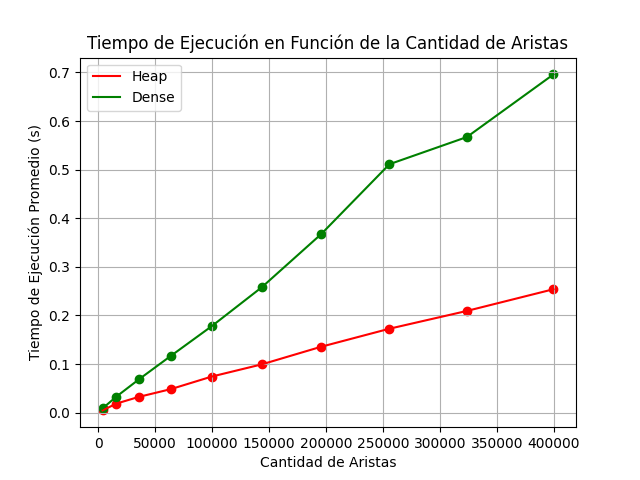
\includegraphics[width=0.7\textwidth, trim=0 0 0 10]{./grafico.png}
    \label{grafico}
\end{figure}

Como puede observarse, el algoritmo de Dijkstra para grafos densos es lineal con respecto a la cantidad de aristas, ya que su complejidad es $O(N^2)$ y la cantidad de aristas también. Para nuestra sorpresa, la implementación basada en heaps (\textit{priority\_queue}), experimentalmente pareciera tener una complejidad $O(N^2)$, cuando teóricamente debería ser $O(N^2 * log(N^2))$. Por un lado, podría ser que el tamaño con el que experimentamos no es suficientemente grande como para denotar una curva en la complejidad. Por otro lado, puede ser que la implementación utilizada para el heap sea tan eficiente que las complejidades de las operaciones de inserción y extracción sean casi constantes en la práctica. Esto podría explicar por qué los tiempos de ejecución del algoritmo para grafos densos sean mayores a pesar de tener una complejidad menor. Eventualmente, para un input suficientemente grande, esta implementación debería ser más rápida para este tipo de grafos.